\documentclass[12pt,a4paper]{article}
\usepackage[utf8]{inputenc}
\usepackage[czech]{babel}
\usepackage[T1]{fontenc}
\usepackage{amsmath}
\usepackage{amsfonts}
\usepackage{amssymb}
\usepackage{color,graphicx}
\usepackage{epstopdf}
\usepackage{indentfirst}
\setlength{\parindent}{4em} 
\author{Jakub Drápela}
\usepackage{fancyhdr}
\usepackage{siunitx}
\usepackage{pdflscape}
\usepackage[backend=bibtex,style=numeric,backref=true]{biblatex}
\definecolor{black}{gray}{0}
\usepackage[pdftex,unicode]{hyperref}
\hypersetup{colorlinks,pdfhighlight=/O,citecolor=black,
  filecolor=black,urlcolor=black,linkcolor=black,
  breaklinks=true,pdfpagemode=UseNone,plainpages=false,
}
\usepackage{filecontents}  % create "citations.bib" on-the-fly
\graphicspath{{./imgs/}}

%\fontfamily{phs}
%\selectfont

\begin{filecontents*}{businessPlan.bib}

@online{pict,
 author  = "The New York Times",
 title   = "The Amazon Echo",
 year    = "2015",
 urlseen = "03-17-16",
 url     = "http://static01.nyt.com/images/2015/06/25/business/GADGETWISE/GADGETWISE-master675.jpg",
}
\end{filecontents*}
\addbibresource{finalReport.bib}

\begin{document}
\pagestyle{empty}

%%nastaveni pisma  
%\fontfamily{phv}
%\selectfont

	\begin{center}

\large

České vysoké učení technické v Praze\\
\medskip
Fakulta elektrotechnická\\[2cm]
{\LARGE\bfseries Household Intelligent Assistant}
\vfill
{\LARGE\bfseries Závěrečná zpráva}
\vfill
\begin{figure}[h!]
\begin{center}
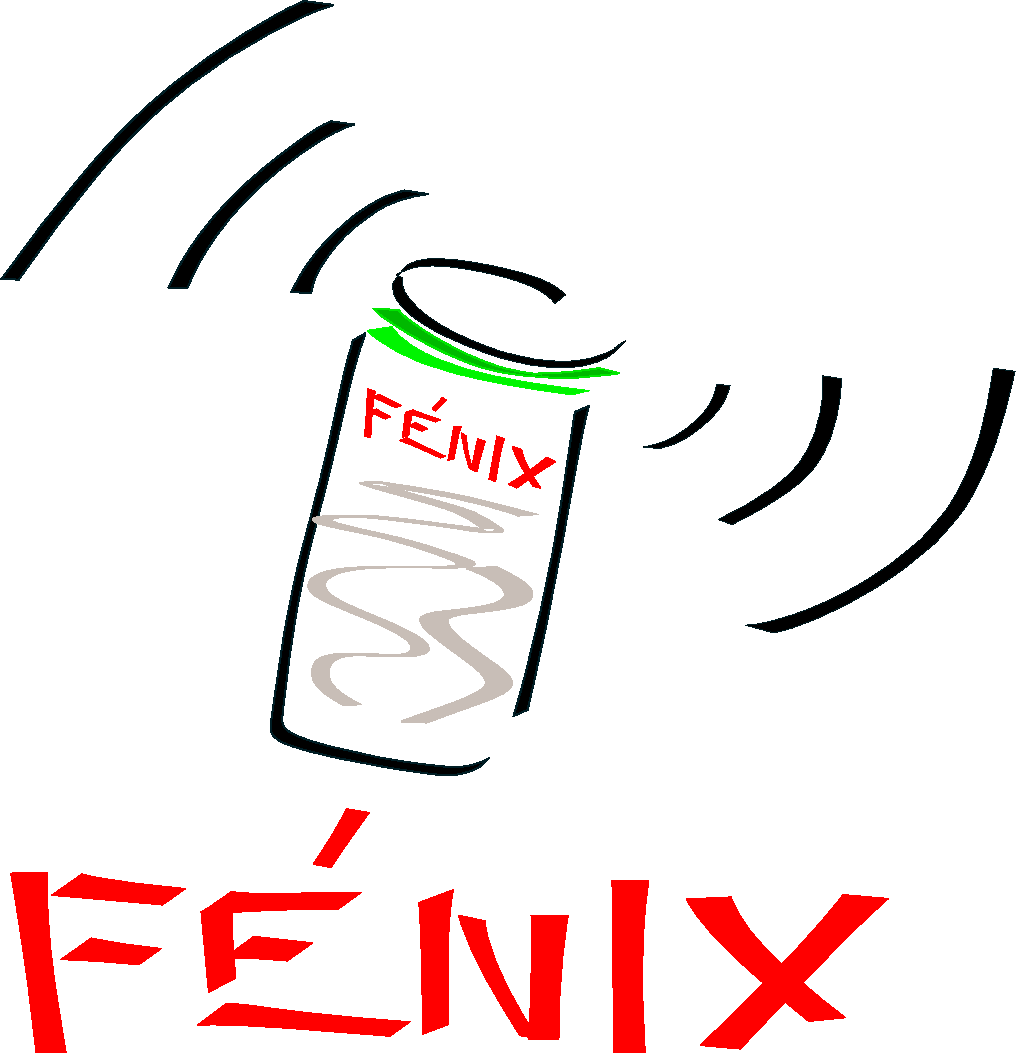
\includegraphics[width = 5cm]{logo.pdf} 
\end{center}
\end{figure}
\vfill

\begin{tabular}{rl}

Autoři: & Jiří Burant \\
\noalign{\vspace{1mm}}
		& Jakub Drápela \\
		\noalign{\vspace{1mm}}
		& Martin Klučka\\
		\noalign{\vspace{1mm}}
		& Petr Kovář \\
		\noalign{\vspace{1mm}}
		& Jakub Konrád\\
		\noalign{\vspace{1mm}}
		& Pavel Trutman\\
\noalign{\vspace{2mm}}
Studijní obor: & Kybernetika a robotika \\
\noalign{\vspace{2mm}}
Datum vypracování: & \today\\
\end{tabular}

\end{center}

\newpage
\pagestyle{plain}     % zapne obyčejné číslování
\setcounter{page}{1}
%% zahlaví a zápatí
\addtolength{\voffset}{-3cm}
\addtolength{\headheight}{2cm}

\pagestyle{fancy}
\lhead{
\includegraphics[scale=0.12]{cvut_text.jpg}  }
\rhead{\textbf{Household Intelligent Assistant}}
%\rhead{\textit{\bfseries Burant,Drápela,Klučka,Kovář,Konrád,Trutman}}
\lfoot{}
\cfoot{\thepage}
\rfoot{}
\renewcommand{\headrulewidth}{0.4pt}

\tableofcontents

\newpage
\section{Úvod}
Cílem této zprávy je provést závěrečné zhodnocení projektu Househol Intelligent Assistant. V rámci zprávy shrneme finální stav produktu a porovnáme dosažené výsledky se zadáním práce. Dále se zaměříme na podrobný popis finálního řešení včetně uvedení milníků. Zároveň připomeneme jednotlivé milníky vývoje, které nás dovedly k finálnímu produktu. 
\section{Finální stav projektu}
Projekt Household Intelligent Assistent se podařilo dokončit v termínu. V současné době existuje beta verze aplikace Househol Intelligent Assistent, která je již plně funkční v rámci zamýšlené domény. Aplikace tedy reaguje na široké spektrum dotazů týkajících se počasí a v omezené podobě také na dotazy z dalších oblastí. Než bude možné vydat oficiální release, je třeba nasbírat více dat od skutečných uživatelů a vyřešit případné dosud neobjevené problémy získane pomocí zpětné vazby. Aktuálně již probíhá uvolnění této beta verze veřejnosti prostřednictvím služby GitHub. Jediným podporovaným systémem, na kterém je aktuálně možné aplikaci spustit, je Linux. 
\section{Popis aplikace}
Aplikace po spuštění vyčkává v stand-by režimu na zaznění klíčového slova “Phoenix”. Jakmile aplikace zaznamená klíčové slovo, uživatel je hlasově upozorněn a může položit zamýšlený dotaz. Dotaz uživatele v mluvené podobě je aplikací převeden na text. Text je dále zpracován za účelem získání záměru. Na základě získaného záměru se vyhledá příslušná odpověď prostřednictvím webové služby. Ze získaných informací je sestavena odpověď a ta je následně prostřednictvím mluveného slova předána uživateli. Na konci tohoto cyklu aplikace  přechází zpět do stand-by režimu a opětovně vyčkává na zaznění klíčového slova.
Prototyp byl důkladně otestován členy týmu a na základě získané zpětné vazby byly jednotlivé moduly laděny tak, aby bylo dosaženo co nejlepších výsledků. Výsledky měření jsou uvedeny v samostatné sekci.

\section{Finální řešení}
Následující sekce stručně popíše finální řešení jednotlivých modulů a součástí projektu


\subsection{Activation word recognition}

\subsection{Speech-to-text}
Ve finální verzi jsme pro Speech-to-text modul využily knihovnu SpeechRecognition, která je napsaná přímo pro programovací jazyk Python. Knihovna využívá pro záznam zvuku knihovnu PyAudio a pro řečovou syntézu může použít více knihoven (CMU Sphinx, IBM Speech To Text, Google Speech Recognition a další). V našem projektu je použitá knihovna od společnosti Google. Knihovna SpeechRecognion pracuje spolehlivě a řečová syntéza je na velmi vysoké úrovni, která splňuje naše stanovené požadavky.

\subsection{Sentence processing}
Tento modul je už od první fáze projektu realizován pomocí aplikace \textit{wit.ai}. Modul přijme dotaz v textové podobě a vrátí strukturovaný objekt obsahující význam daného dotazu. Aplikace \textit{wit.ai} porovnává dotaz s námi vytvořenou databází a vrátí význam vyhodnocený jako nejpřesnější shodu spolu s "confidence score", pomocí kterého následující moduly určí, zda je dotaz validní, či ne.

\subsection{Data query a Answer formulation}
Modul, který obstarává vyhledávání informací a logiku, která má být vykonána na základě intentu se nazývá \textit{querylogic}. Tento modul dostane od jádra jako vstup zpracovaný dotaz z \textit{Wit.ai} a podle jeho významu vykoná žádané úkony a vyhledá potřebné informace. Následně vrátí zpět do jádra sestavenou odpověď ve formě textového řetězce.

Hlavní částí modulu querylogic je obsluha dotazů z oblasti počasí.  Modul je schopen poskytnout historické informace o počasí a týdenní předpověď počasí pro různá místa na zemi, pokud má potřebná data k dispozici. Ve finální verzi je implemetován souhrn počasí za určitý časový interval, který v předchozí verzi chyběl. Nyní je možné ptát se nejen na předpověď pro daný den a čas, ale také na časový interval a modul shrne celou předpověď do stručné odpovědi.

Byl dokončen submodul obecné komunikace, který je schopen obstarávat dotazy na čas a vybírat vtipné fráze z vlastní databáze.

Dále byl vytvořen jednoduchý submodul, který je schopen vyhledat aktuální noviky ze světa.

Zároveň jsou v modulu qeurylogic odfiltrovány dotazy, ke kterým \textit{Wit.ai} přiřadí nepodporovaná význam, a na které tedy  modul není schopen správně odpověďet a také dotazy s "confidence score" pod nastaveným prahem. Prahové hodnoty pro rozhodnutí byly získány pomocí testovaání sady žádoucích a nežádoucích dotazů.

\subsection{Text-to-speech}
V modulu \textit{text-to-speech} nedošlo v poslední fázi projektu k výrazným změnám. Modul využívá syntetizátor řeči \textit{Mimic} od společnosti \textit{Mycroft}. 
Kvalita syntetizované řeči není sice srovnatelná s komerečním softwarem a je patrné, že řeč je strojové povahy, ale je plně srozumitelná a pro naše použití tak dostačující.


\section{Stav projektu v rámci časového plánu}
Jak již bylo řečeno v úvodu, projekt se podařilo dokončit dle sestaveného harmonogramu. V současné době tedy máme plně funkční aplikaci testovanou interně mezi členy týmu, kterou od oficiálního releasu děli už jen plánované testování komunitou uživatelů. Vzhledem k neočekávaným problémům týkajících se modulu pro převod řeči na text, které si vyžádaly plné nasazení všech členů týmu, bylo nutné zkrátit testovací dobu z plánovaných tří týdnů na dva. Díky přeorganizaci týmu se nám povedlo zamýšlené testování provést i v tomto zkráceném čase.

\section{Testy a zhodnocení výkonu}
Projekt prošel několika testovacímí fázemi. Kromě běžného testovaní funkcionality jednotlivých programových součástí všech modulů, jsme navrhli experimet pro otestování každého z modulů \textit{Activation word}, \textit{Speech-to-text} a \textit{Sentence processing}. K samostatnému testování byly vybrány tyto moduly, protože právě na nich závisí, zda náš systém spracuje dotaz uživatele, a má smysl u nich mluvit o úspěšnosti. Dále byl systém otestován jako celek, tedy od zavolání systému pomocí attention word až po jeho odpověď.




\subsection{Activation word recognition - testování}
Moduly závisející na speech recognition, tedy \textit{Activation word} a \textit{Speech-to-text} byly testovány ve dvou prostředích a to v místnosti bez echa a běžného akustického pozadí (klidná místnost) a poté v běžném prostření akustickým pozadím (hlučná místnost). 

Modul byl testován ve dvou fázích. Nejprve byl vždy osloven pomocí klíčového slova, a bylo zaznamenáno, zda úspěšně zareagoval, či ne a poté byl ponechán aktivní a bylo v jeho tesnována jeho falešně pozitivní reakce. 

V blízkosti mikrofonu jsme se bavili 15 minut v anglickém jazyce a 15 minut v českém jazyce. Dále jsme zkoušeli systém oslovovat slovy podobnými aktivačnímu "\textit{Phoenix}".

 Testování se účastnili vždy 3 muži ve věku 20-25 let a proběhlo 125 dotazů na klíčové slovo pro klidnou místnost a 60 dotazů pro hlučnou místnost.
 
Při testech rozpoznání klíčového slova v klidné místnosti jsme měli celkovou úspěšnost 86 \%. K falošně pozitivní detekci došlo pouze jednou.  Výsledek testu je znázorněn na grafu \ref*{fig:AttentionWord}.

	\begin{figure}[ht]
		
		\centering
		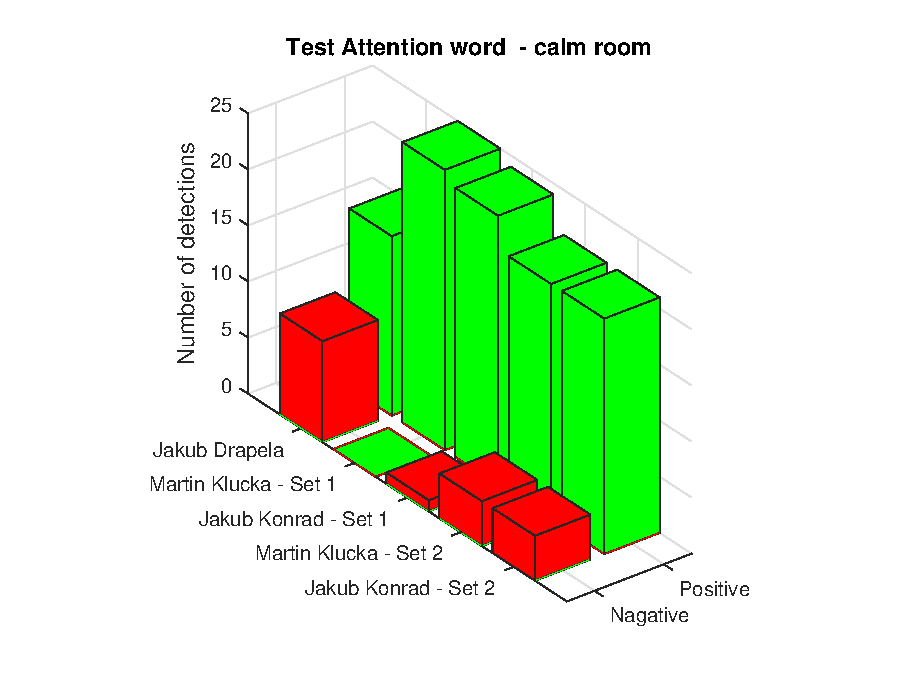
\includegraphics[width = 12cm]{AtWr_test.eps}
		\caption{Výsledky rozpoznání klíčového slova na 3 respondentech v klidné místnosti.}
		\label{fig:AttentionWord}
	\end{figure}
	
V hlučné místnosti s ozvěnou jsme byli schopni naším systémem detekovat 80 \% dotazů s klíčovým slovem. Objevili se také falešné detekce, ke kterým došlo celkem 4-krát během celého testování Výsledek testu je znázorněn na grafu \ref*{fig:AttentionWord2}. 

	\begin{figure}[ht]
		
		\centering
		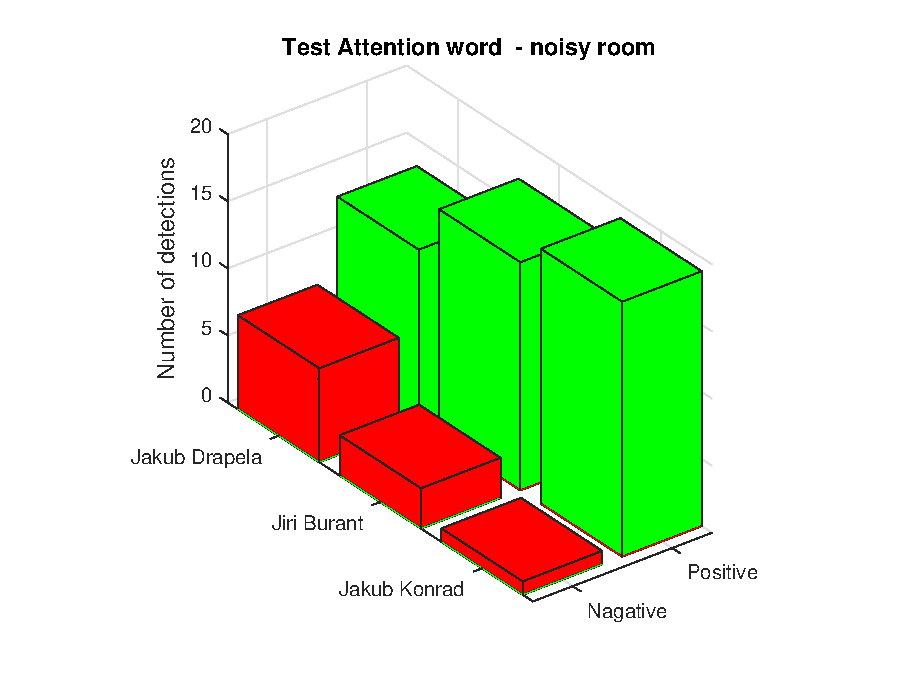
\includegraphics[width = 12cm]{AtWr_test2.eps}
		\caption{Výsledky rozpoznání klíčového slova na 3 respondentech v hlučné místnosti.}
		\label{fig:AttentionWord2}
	\end{figure}

\subsection{Speech-to-text - testování}
Modulu bylo v obou verzích testu prředloženo 60 dotazů a ze získaných odpovědí byla vyhodnocená jeho přesnost. Výsledky byly rozděleny do tří kategorií - správně vyhodnocené dotazy, dotazy s drobnými odchylkami (zorpoznáno "is" místo "was", špatně rozpoznaný místní název jako Liberec nebo Krkonoše), které leze pro naše účely s ohledem na možnosti systému stále považovat za správně vyhodnocené a dozaty vyhodnocené nesprávně.
Výsledny testů je možno vidět v grafu na obrázku.
 \ref*{fig:speech}.
\begin{figure}[ht]
	\begin{center}
		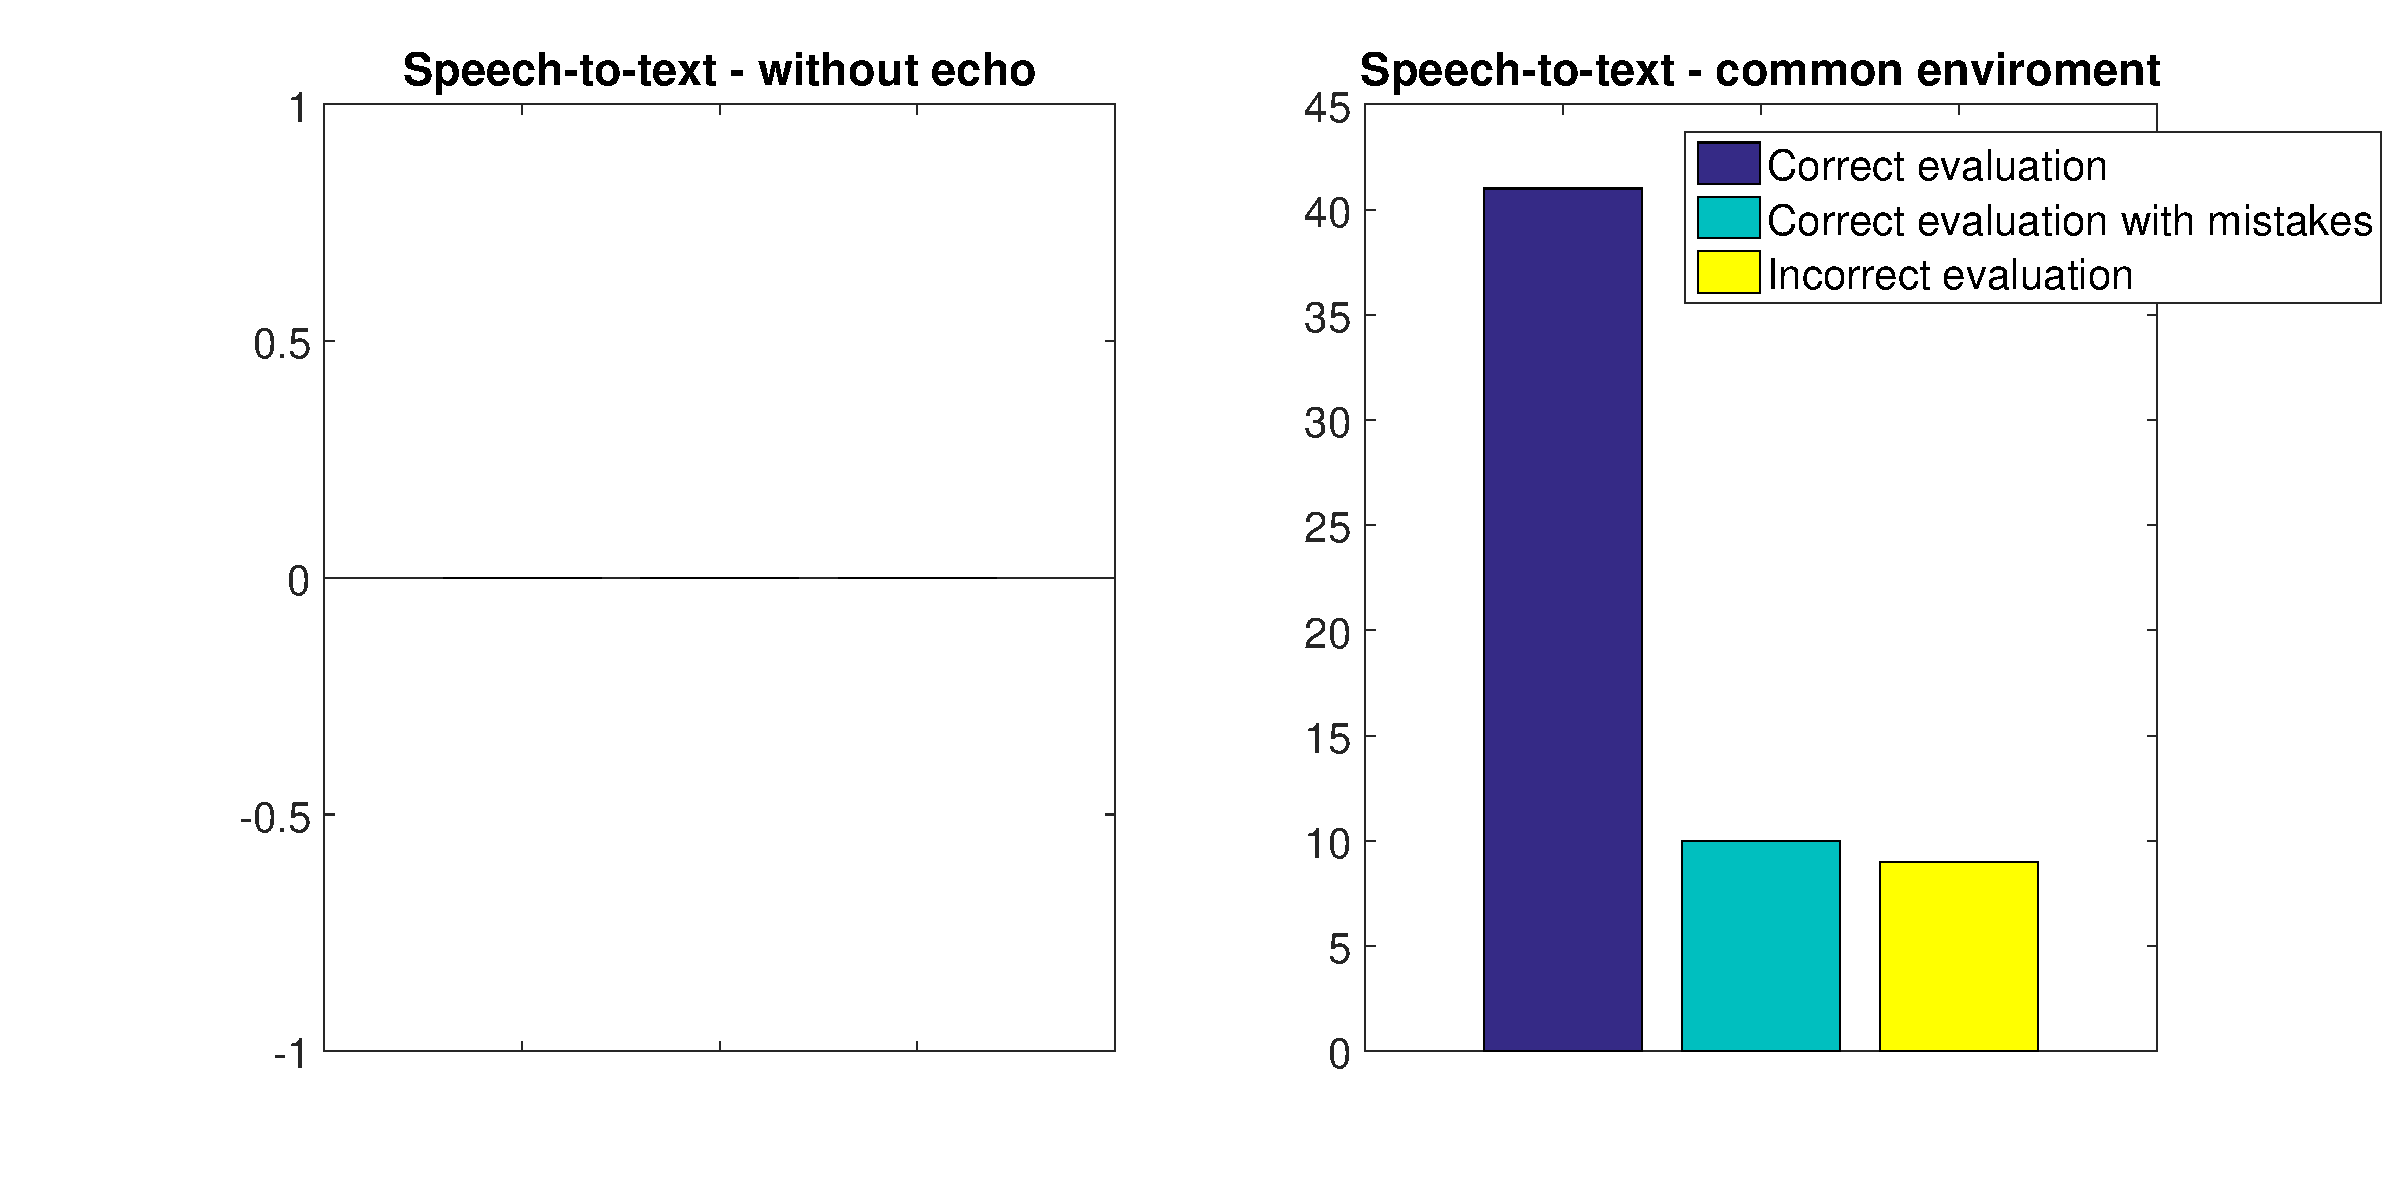
\includegraphics[width = 1\textwidth ]{stt.eps}
		\caption{Výsledky testování modulu Speech-to-text.}
		\label{fig:speech}
	\end{center}
\end{figure}


Pro testování v běžném prostření lze pozorovat nepatrné zhoršení výsledků, tedy 51 dozazů bylo správně vyhodnoceno a 9 dozazů bylo špatně vyhodnoceno. 
Tuto úspěšnost považujeme za velmi dobrý výsledek pro oba experimenty.

Při testování jsme navíc zjistili, pravděpodobnost rozpoznání dotazu zvyšuje správná artikulace a dostatečná hlasitost řeči. 

\subsection{Sentence processing - testování}
Modul \textit{Sentence processing} byl otestován pomocí vytvořené sady testovacích dotazů. Výsledky modulu byly porovnány se zamýšlenými výsledky sady a následně vyhodnoceny.
Testovací sada se obsahovala 70 dotazů a obsahovala jak dotazy na které má systém umět odpovědět, tak dotazy které jsou mimo scope systému. Pokud systém odpověděl dle očekávání, byl dotaz vyhodnocen jako správně zodpovězený. Pokud se systém odlišil, odpověď byla vyhodnocena jako špatná. Výsledky systému lze vidět na níže uvedeném grafu (obrázek \ref*{fig:sentence_processing}).

\begin{figure}[ht]
	\begin{center}
		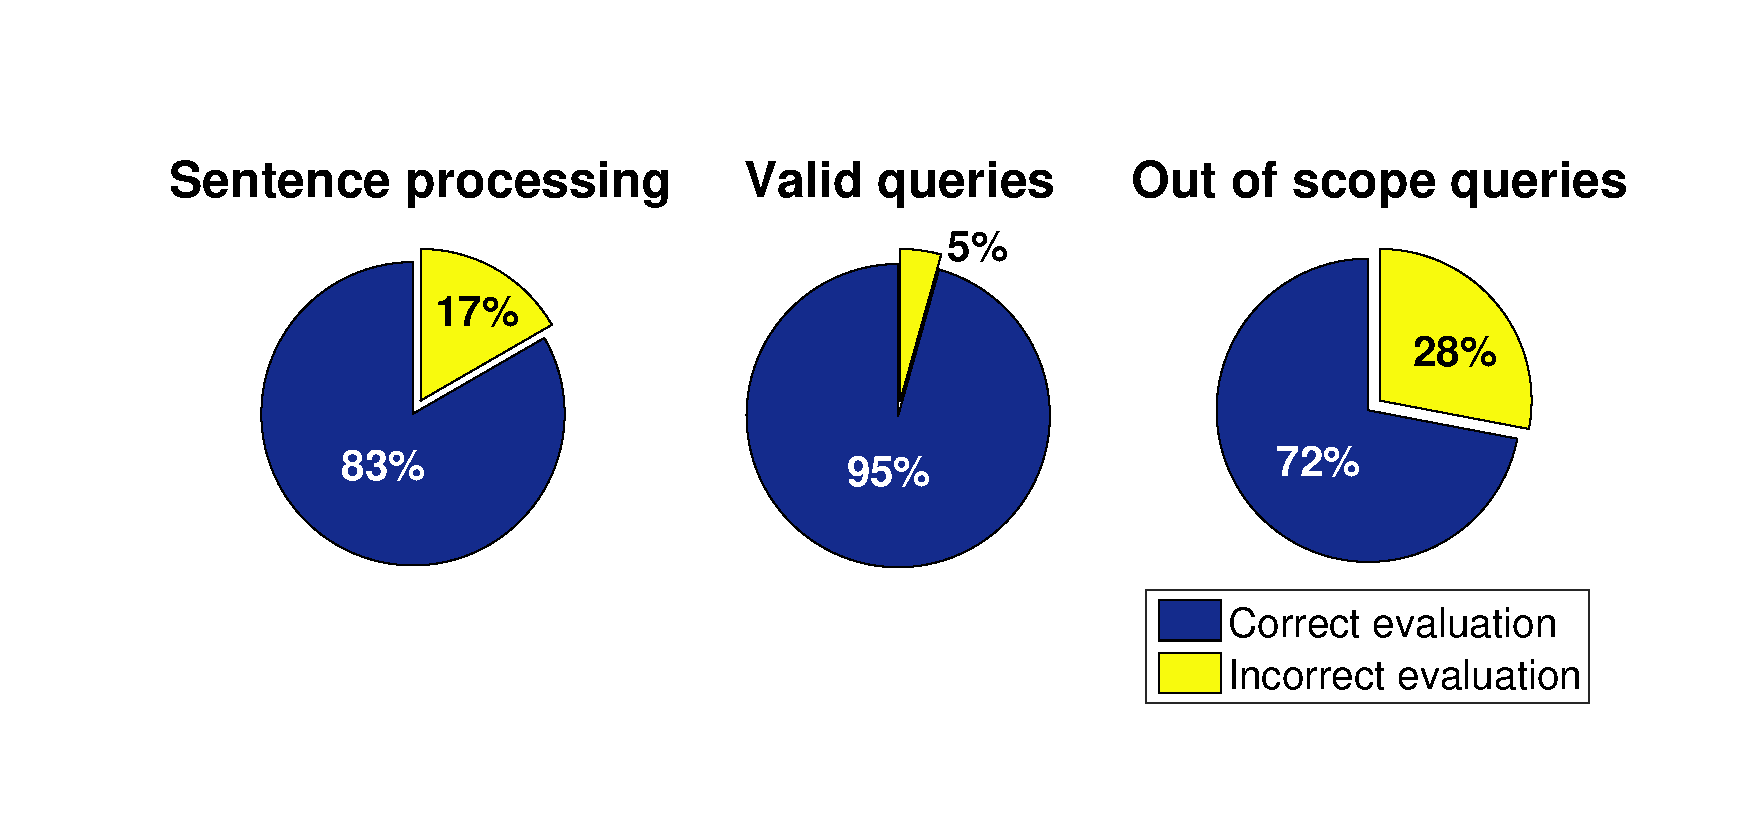
\includegraphics[width = 1\textwidth ]{sentence.eps}
		\caption{Výsledky testování modulu sentence processing.}
		\label{fig:sentence_processing}
	\end{center}
\end{figure}

Z výsledků lze pozodovat, že pro validní dotazy dosahuje náš systém velmi vysoké úspěšnosti - až 95 procent. Pro dotazy, na které systém neumí odpovědět lze pozorovat zvýšenou míru falešně pozotovních vyhodnocení. TOto je způsoveno zatím neimplementovanou podporou pro filtraci nepodporovaných významů v nástroji \textit{wit.ai}. I přes tento nedostatek se nám podařilo dosáhnout správného rozpoznání nevalidního dotazu v 72 procentech případů.

\subsection{Testování celého systému}
Následující test byl proveden v běžném prostření akustickým pozadím. Systém byl testován stejným způsobem, jakým by jej používal běžný uživatel, tedy byl zavolán, byla mu položena otázka a byla zaznamenána odpověď. Celý průběh jednoho dotazu byl poté vyhodnocen. Systém byl dotázán celkem 45-krát.

\begin{figure}[ht]
	\begin{center}
		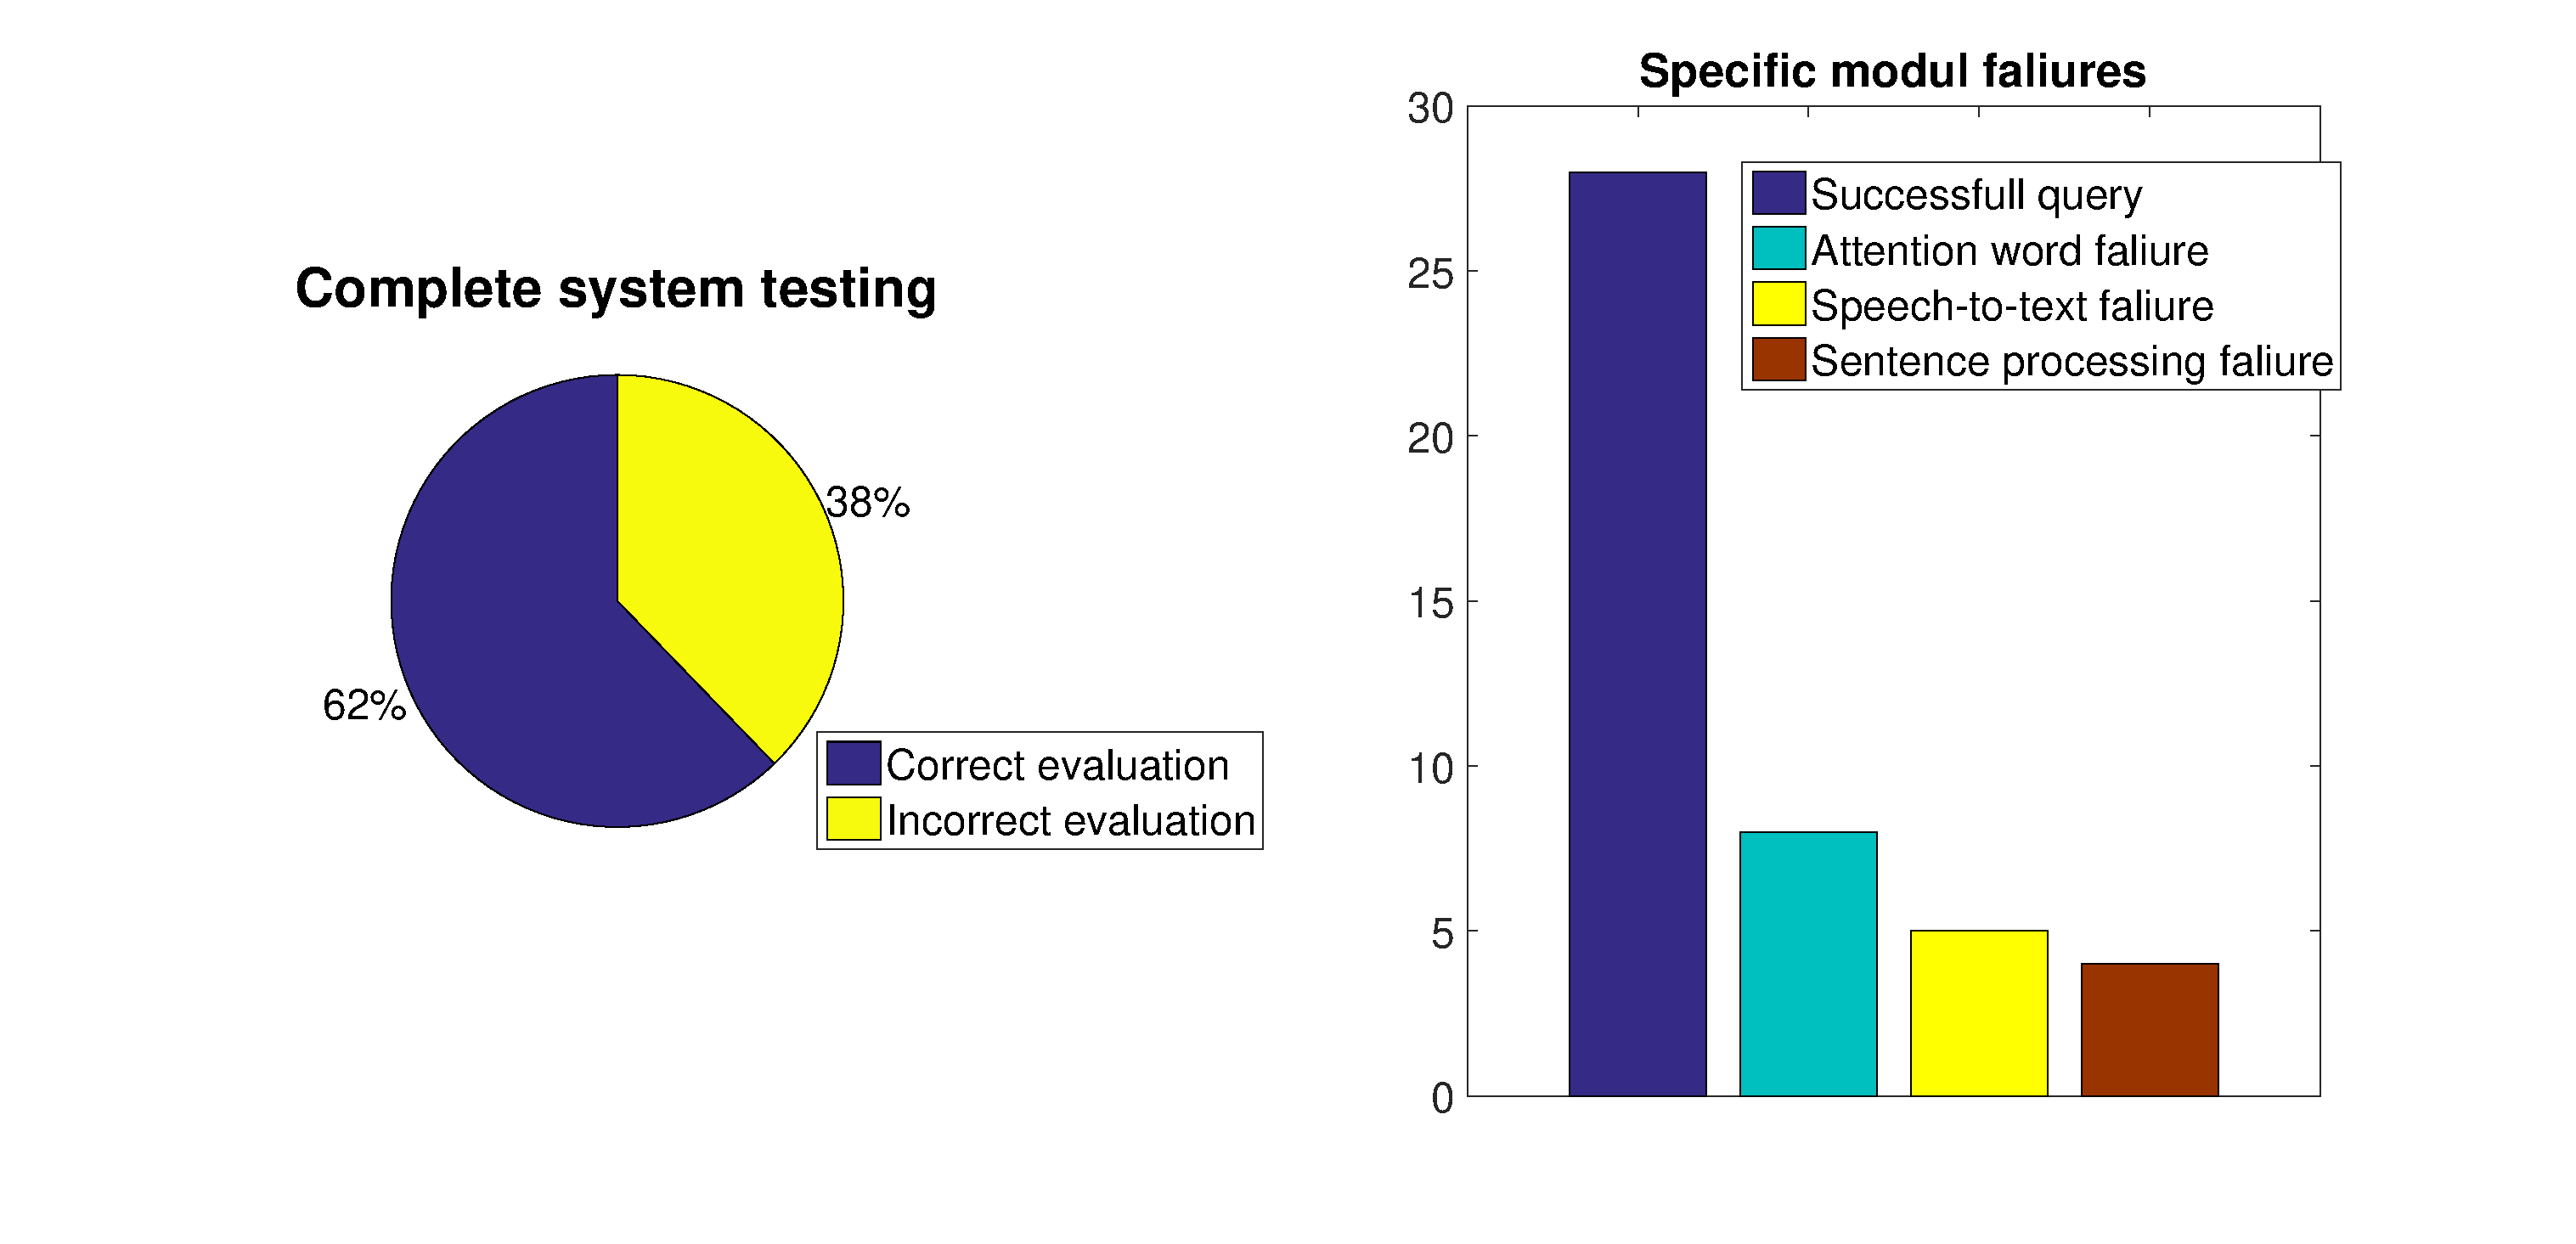
\includegraphics[width = 1\textwidth ]{full.eps}
		\caption{Výsledky testování celého systému.}
		\label{fig:full}
	\end{center}
\end{figure}

V grafu \ref*{fig:full} vidíme, že systému se podařilo odpovědět na položený dotaz v 62 procentech případů. Tato úspěšnost je poměrně nízká, je však potřeba vzít v úvahu, že z 17 neúspěšných testů jich 8 selhalo na oslovení systému, v tomto přípahě uživatel systém pouze osloví znovu a po úspěšné registraci klíčového slova může pokračovat. Pokud bychom vypostili testy, kde bylo první oslovení systému neúspěšné, dostali bychom se s úspěšností na 75 procent, což už se jeví jako přijatelnější výsledek.

\subsection{Shrnutí výsledků testů}
Souhrnně lze říci, že výsledky testů systému byly pozitivní. Jednotlivé moduly si vedly velmi dobře. Systém jako celek má výsledky horší, ale stále přijatelné.

Věříme, že s dostatkem času je možné výsledky systému zlepšit a systém zrobustnit tak, aby se jeho selhání stalo pouze ojedinělým jevem.



\section{Jak náš projekt vyzkoušet a otestovat}

\section{Závěrečné zhodnocení projektu}


\begin{landscape}
~\vfill
\begin{figure}[ht]
	\begin{center}
	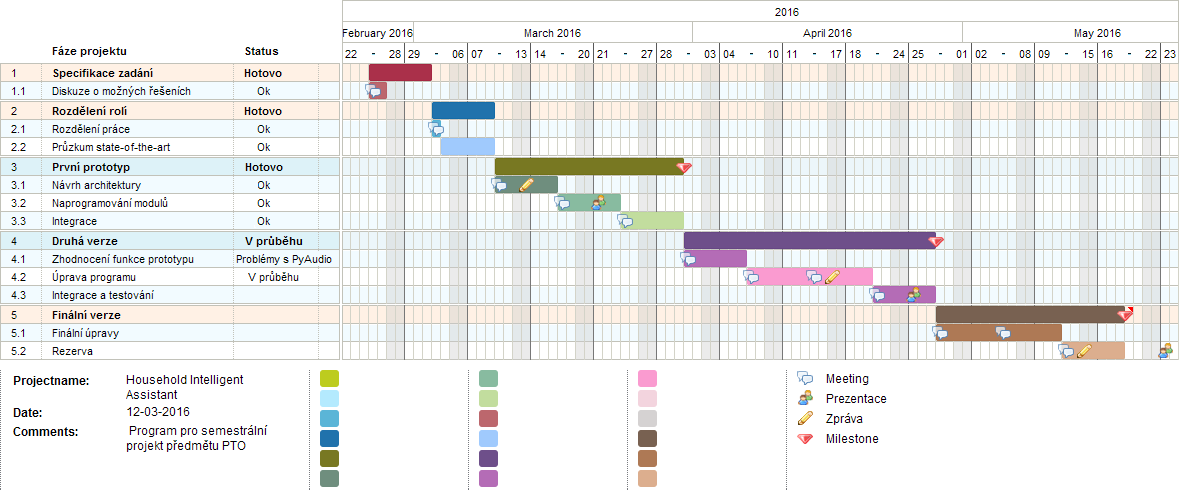
\includegraphics[height = 0.6\textheight ]{PTO-Gantt.png}
	\caption{Harmonogram projektu graficky znázorněn formou Ganttova diagramu s klíčovými milníky.}
	\label{fig:diagram_gantt}
	\end{center}
\end{figure}
\vfill
\end{landscape}

\end{document}
